\section{Experiments}

\subsection{Matrix Generation and Results}
We use several functions to generate those matrices we need to do this experiment.
\begin{lstlisting}[language=Matlab, caption=generating matrices with the specified condition number]
function A = genMatrix(size, cond)
    A = 2*rand(size);
    [u, s, v] = svd(A);
    s = diag(s);
    s = s(1)*( 1-((cond-1)/cond)*(s(1)-s)/(s(1)-s(end))) ;
    s = diag(s);
    A = u*s*v';
end
\end{lstlisting}
Small size matrices:
\begin{lstlisting}[language=Matlab, caption=Small size mtrix]
    cond = [1e2, 1e3, 1e4, 1e5, 1e6, 1e7, 1e8, 1e9];
matrices = cell(size(cond,2));
for i=1:size(cond,2)
    matrices{i} = genMatrix(500, cond(i));
end

relresgm = zeros(size(matrices,2),1);
relreslu = zeros(size(matrices,2),1);
itergm = zeros(size(matrices,2),1);
iterlu = zeros(size(matrices,2),1);
timegm = zeros(size(matrices,2),1);
timelu = zeros(size(matrices,2),1);

for i = 1:size(matrices,2)
    b = rand(size(matrices{i},1),1);
    tic
    [x, flag, relres, iter] = gmres(matrices{i}, b, [], 1e-6, 30);
    timegm(i) = toc;
    relresgm(i) = relres;
    flags(i) = flag;
    itergm(i) = iter(2);

    tic
    [x, relres, iter] = iterref(matrices{i}, b);
    timelu(i) = toc;
    relreslu(i) = relres(size(relres,2));
    iterlu(i) = iter;
end

figure(1)
semilogy(cond, relreslu);
title("luir: accuracy vs condition (small matrix - 500x500)")
saveas(gcf,'luir_acc_smat.png')
figure(2)
semilogy(cond, relresgm);
title("gmres: accuracy vs condition (small matrix - 500x500)")
saveas(gcf,'gmres_acc_smat.png')

figure(3)
plot(cond, iterlu);
title("luir: iterations vs condition (small matrix - 500x500)")
saveas(gcf,'luir_iter_smat.png')
figure(4)
plot(cond, itergm);
title("gmres: iterations vs condition (small matrix - 500x500)")
saveas(gcf,'gmres_iter_smat.png')

figure(5)
plot(sizes, timelu);
title("luir: time vs matrix size (low condition number)")
saveas(gcf,'luir_acc_lcond.png')
figure(6)
plot(sizes, timegm);
title("gmres: time vs matrix size (low condition number)")
saveas(gcf,'luir_acc_lcond.png')

\end{lstlisting}  
With these small matrices, we got the results as below:
\begin{figure}[ht]
     \begin{minipage}[b]{0.5\linewidth}
        \centering
   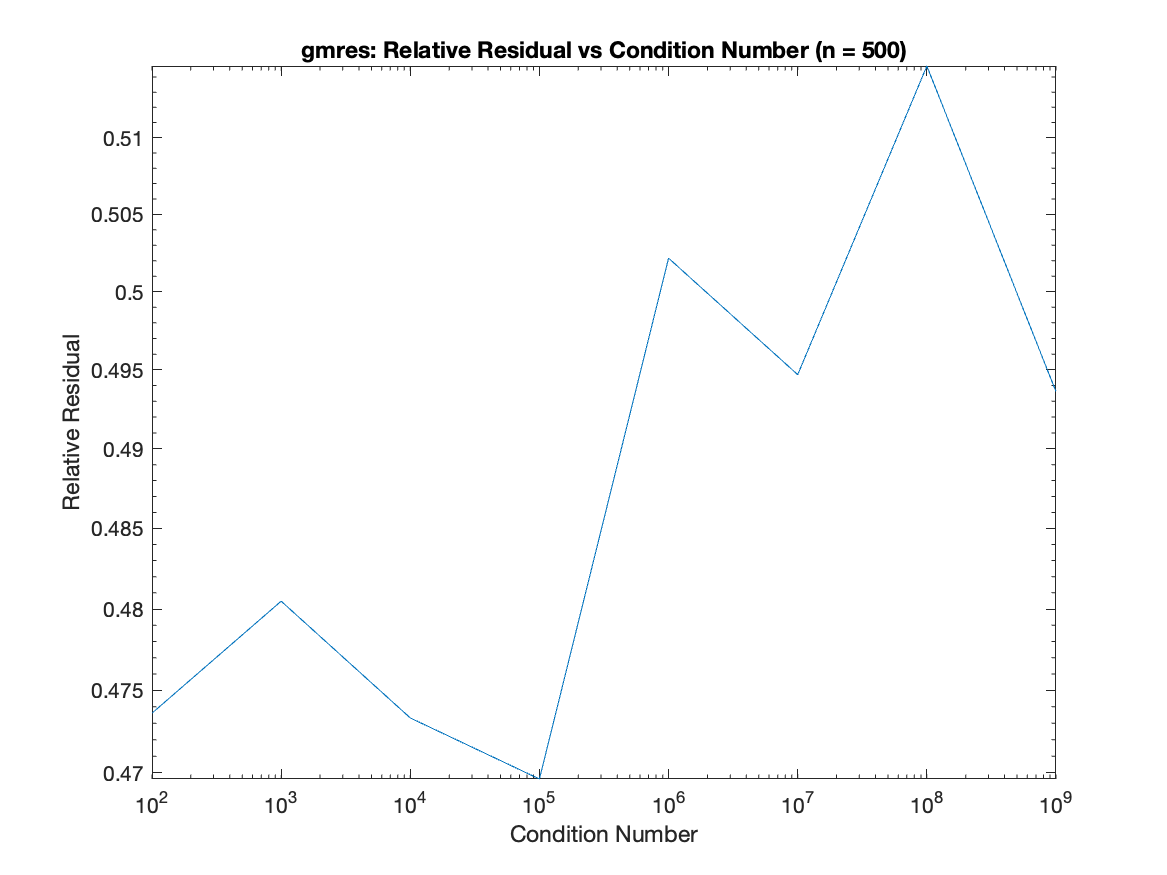
\includegraphics[width=\linewidth]{Plot/gmres_acc_smat.png}
        \caption{Accuracy with condition number with GMRES}
        \label{fig:image1}
    \end{minipage}
    \hspace{0.5cm} 
    \begin{minipage}[b]{0.5\linewidth}
        \centering
        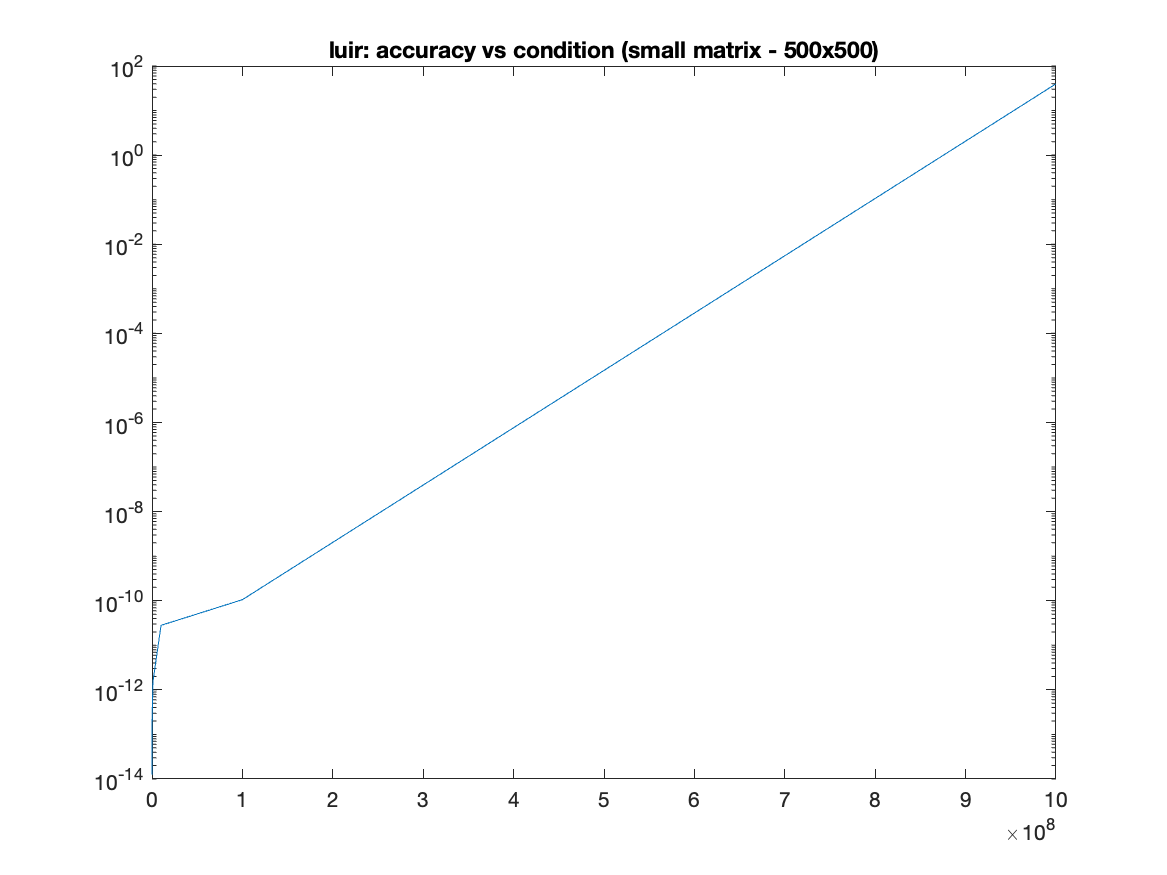
\includegraphics[width=\linewidth]{Plot/luir_acc_smat.png}
        \caption{Accuracy with condition number with LU-IR.}
        \label{fig:image2}
    \end{minipage}
\end{figure}

\begin{figure}[ht]
     \begin{minipage}[b]{0.5\linewidth}
        \centering
   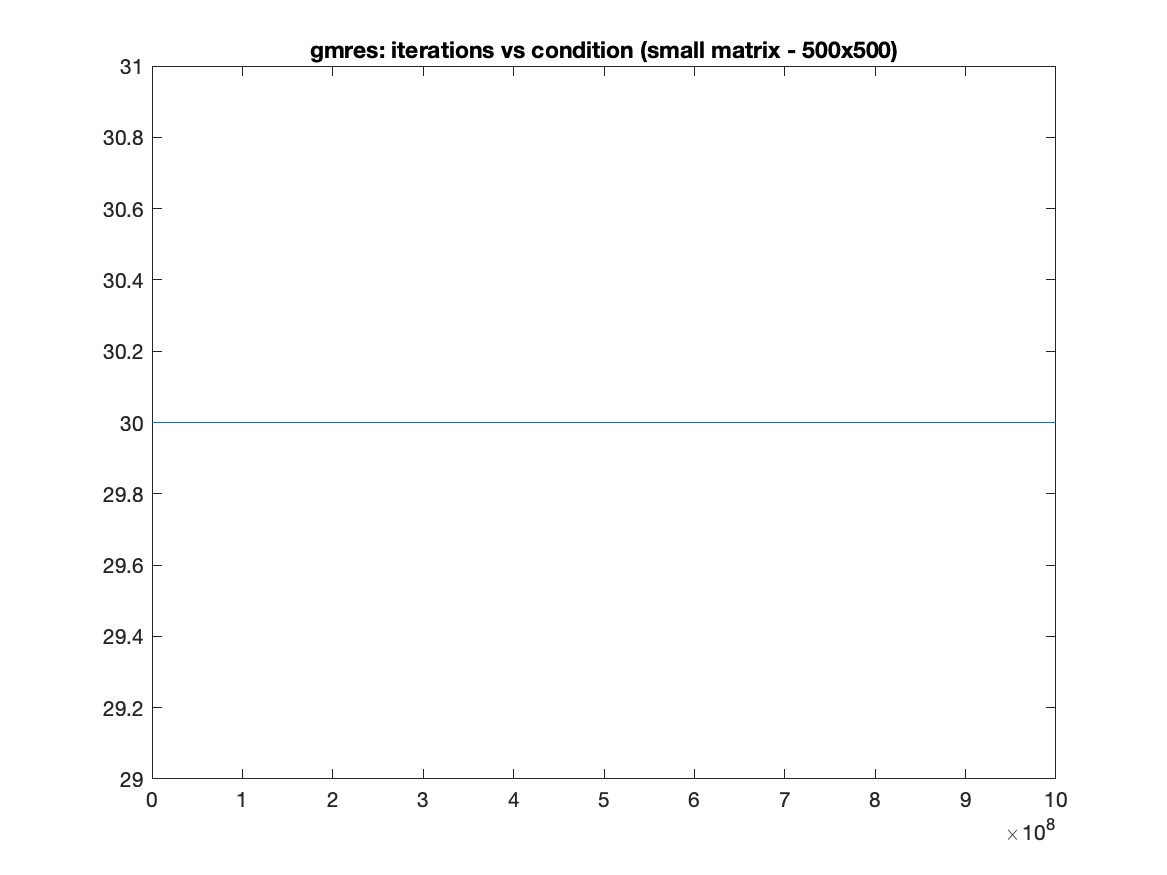
\includegraphics[width=\linewidth]{Plot/gmres_iter_smat.png}
        \caption{Iterations with condition number with GMRES}
        \label{fig:image3}
    \end{minipage}
    \hspace{0.5cm} 
    \begin{minipage}[b]{0.5\linewidth}
        \centering
        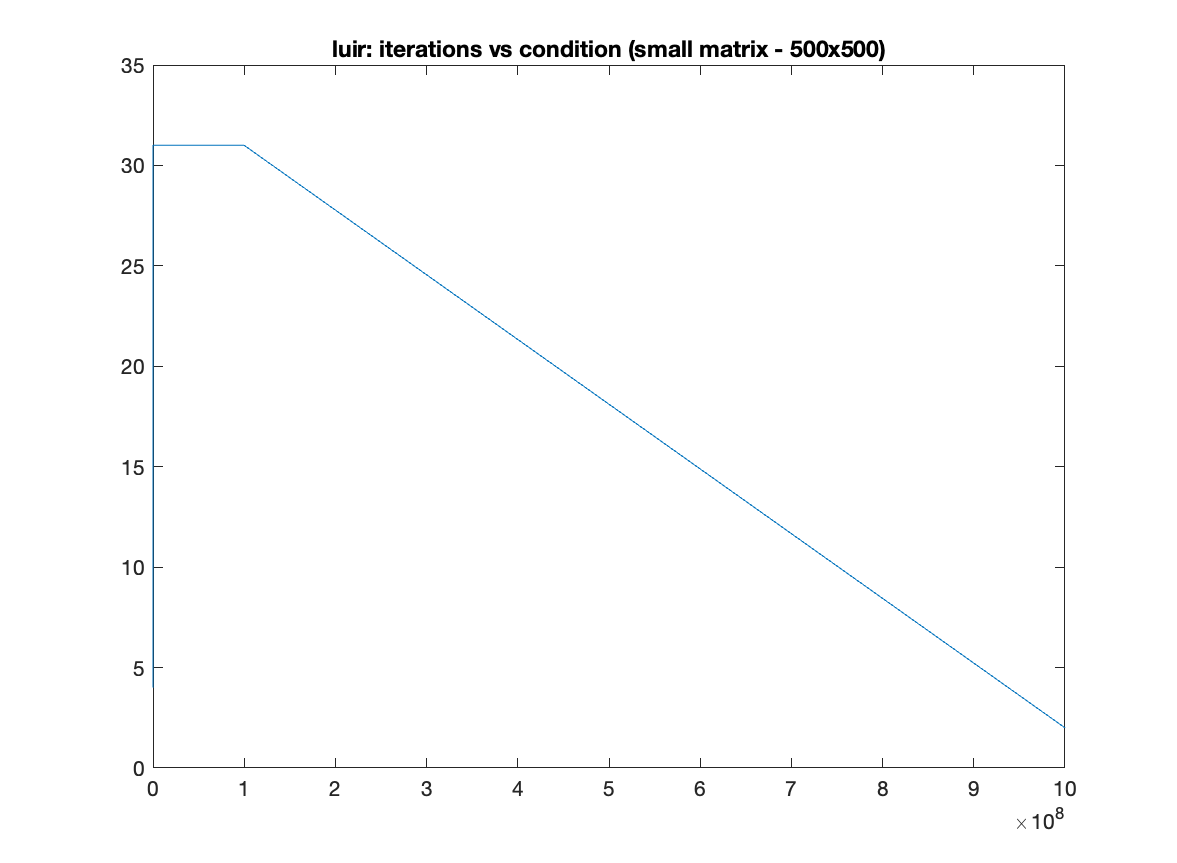
\includegraphics[width=\linewidth]{Plot/luir_iter_smat.png}
        \caption{Iterations with condition number with LU-IR.}
        \label{fig:image4}
    \end{minipage}
\end{figure}
\newpage
\begin{figure}[ht]
     \begin{minipage}[b]{0.5\linewidth}
        \centering
   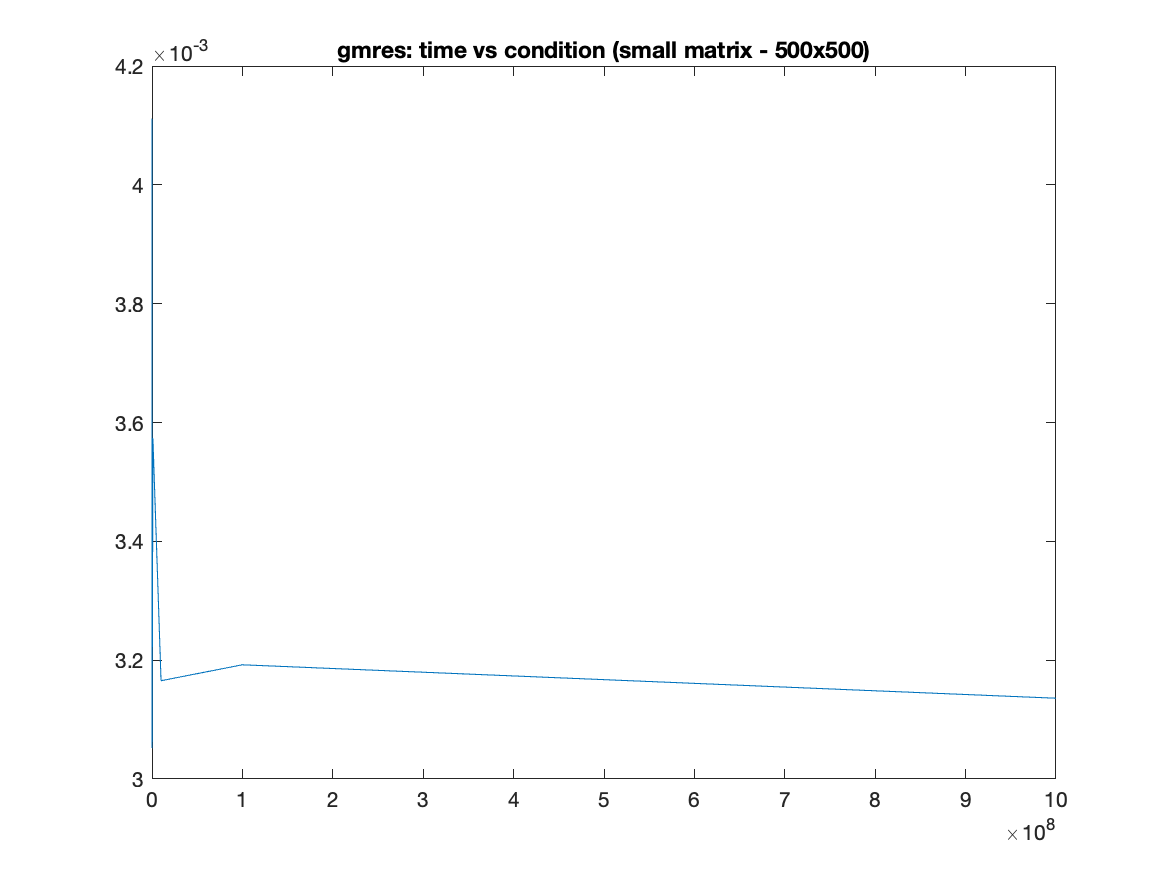
\includegraphics[width=\linewidth]{Plot/gmres_time_smat.png}
        \caption{Time with condition number with GMRES}
        \label{fig:image5}
    \end{minipage}
    \hspace{0.5cm} 
    \begin{minipage}[b]{0.5\linewidth}
        \centering
        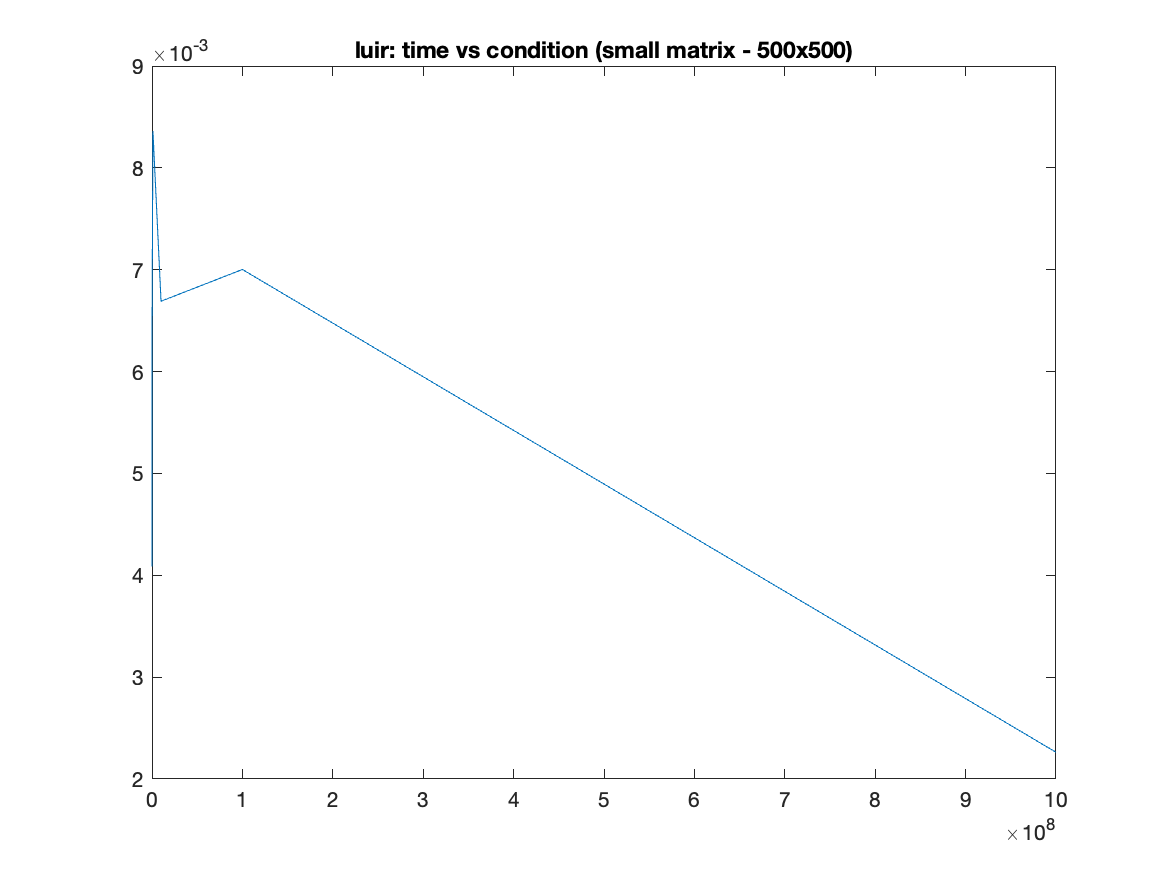
\includegraphics[width=\linewidth]{Plot/luir_time_smat.png}
        \caption{Time with condition number with LU-IR.}
        \label{fig:image6}
    \end{minipage}
\end{figure}

\clearpage
\newpage
Large size matrices:
\begin{lstlisting}[language=Matlab, caption=Large size matrix]
    cond = [1e2, 1e3, 1e4, 1e5, 1e6, 1e7, 1e8, 1e9];
matrices = cell(size(cond,2));
for i=1:size(cond,2)
    matrices{i} = genMatrix(5000, cond(i));
end

relresgm = zeros(size(matrices,2),1);
relreslu = zeros(size(matrices,2),1);
itergm = zeros(size(matrices,2),1);
iterlu = zeros(size(matrices,2),1);
timegm = zeros(size(matrices,2),1);
timelu = zeros(size(matrices,2),1);
flags = zeros(size(matrices,2),1);

for i = 1:size(matrices,2)
    b = rand(size(matrices{i},1),1);
    tic
    [x, flag, relres, iter] = gmres(matrices{i}, b, [], 1e-6, 30);
    timegm(i) = toc;
    relresgm(i) = relres;
    flags(i) = flag;
    itergm(i) = iter(2);

    tic
    [x, relres, iter] = iterref(matrices{i}, b);
    timelu(i) = toc;
    relreslu(i) = relres(size(relres,2));
    iterlu(i) = iter;
end

figure(1)
semilogy(cond, relreslu);
title("luir: accuracy vs condition (large matrix - n=10000)")
saveas(gcf,'luir_acc_lmat.png')
figure(2)
semilogy(cond, relresgm);
title("gmres: accuracy vs condition (large matrix - n=10000)")
saveas(gcf,'gmres_acc_lmat.png')

figure(3)
plot(cond, iterlu);
title("luir: iterations vs condition (large matrix - n=10000)")
saveas(gcf,'luir_iter_lmat.png')
figure(4)
plot(cond, itergm);
title("gmres: iterations vs condition (large matrix - n=10000)")
saveas(gcf,'gmres_iter_lmat.png')

figure(5)
plot(sizes, timelu);
title("luir: time vs matrix size (low condition number)")
saveas(gcf,'luir_acc_lcond.png')
figure(6)
plot(sizes, timegm);
title("gmres: time vs matrix size (low condition number)")
saveas(gcf,'luir_acc_lcond.png')

\end{lstlisting}
With large matrices as above, we got those results as below:
\begin{figure}[ht]
     \begin{minipage}[b]{0.5\linewidth}
        \centering
   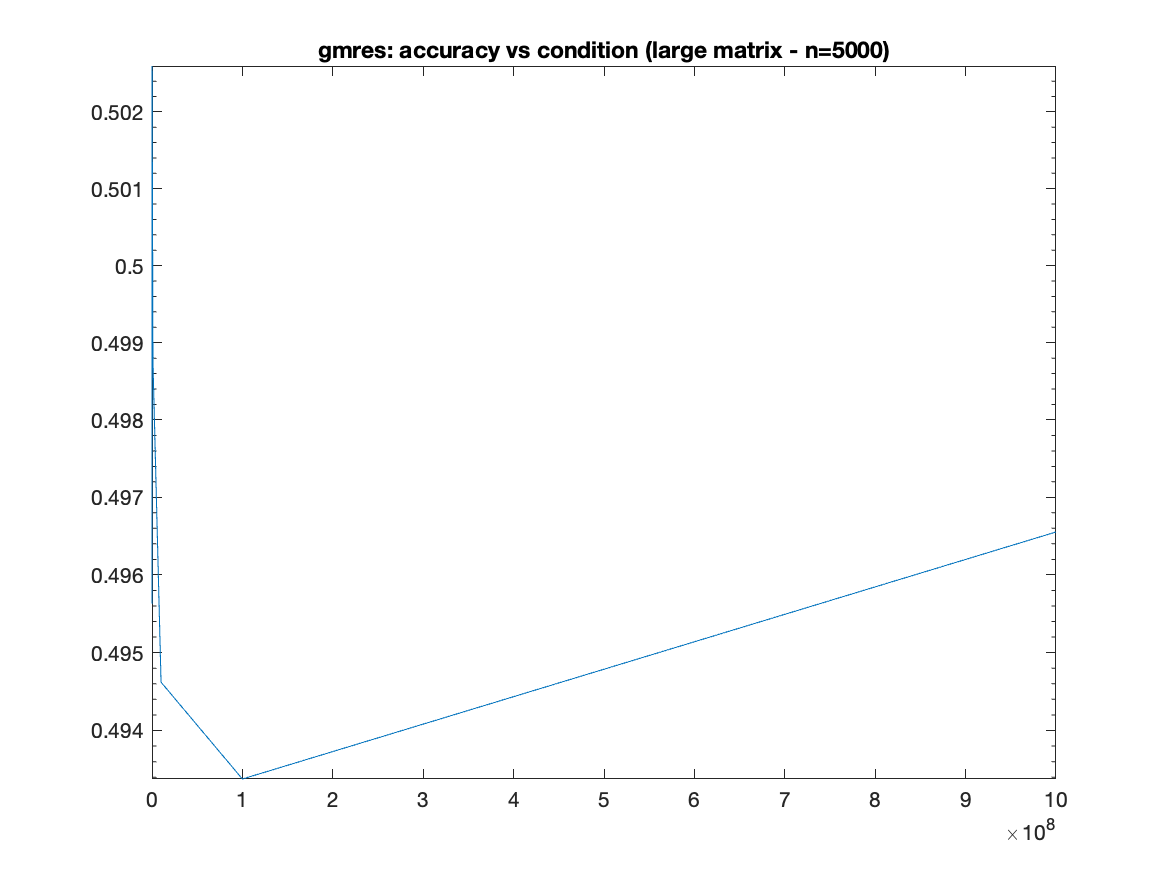
\includegraphics[width=\linewidth]{Plot/gmres_acc_lmat.png}
        \caption{Accuracy with condition number with GMRES}
        \label{fig:image7}
    \end{minipage}
    \hspace{0.5cm} 
    \begin{minipage}[b]{0.5\linewidth}
        \centering
        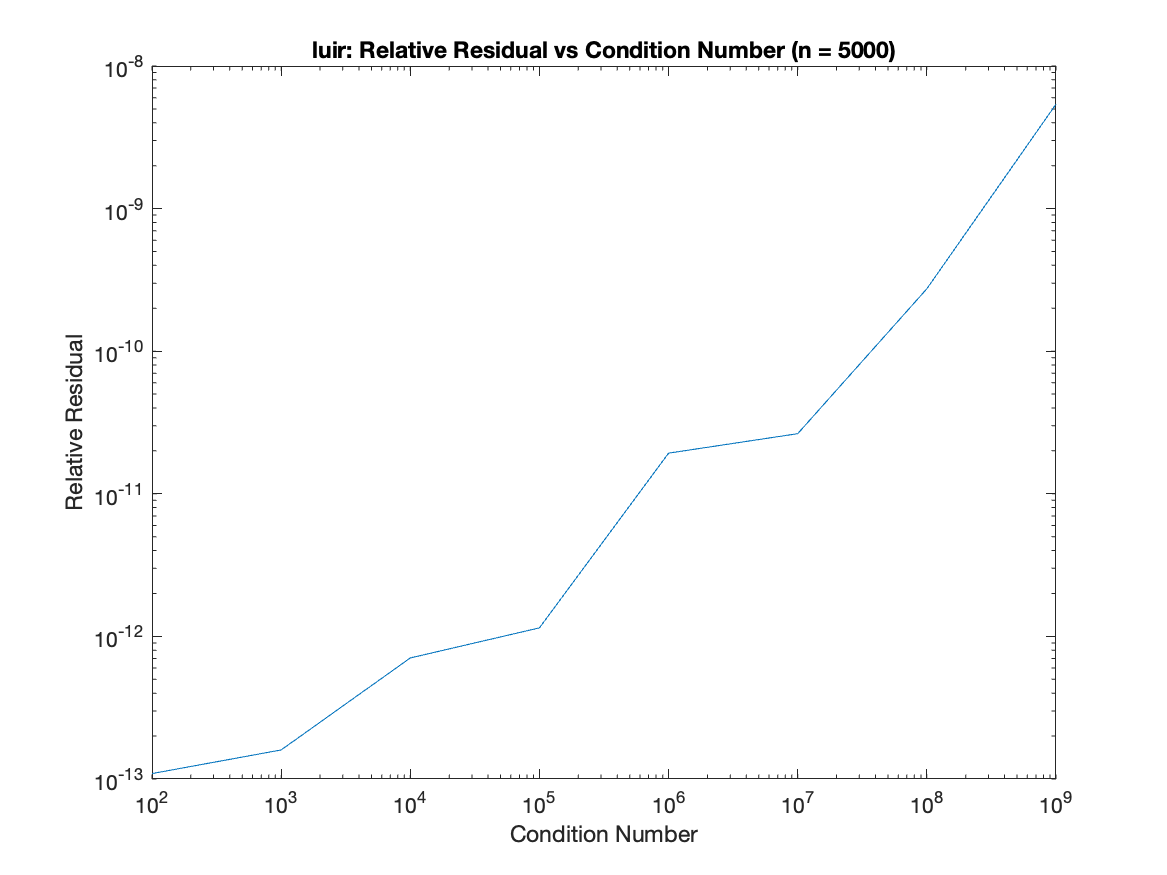
\includegraphics[width=\linewidth]{Plot/luir_acc_lmat.png}
        \caption{Accuracy with condition number with LU-IR.}
        \label{fig:image8}
    \end{minipage}
\end{figure}

\begin{figure}[ht]
     \begin{minipage}[b]{0.5\linewidth}
        \centering
   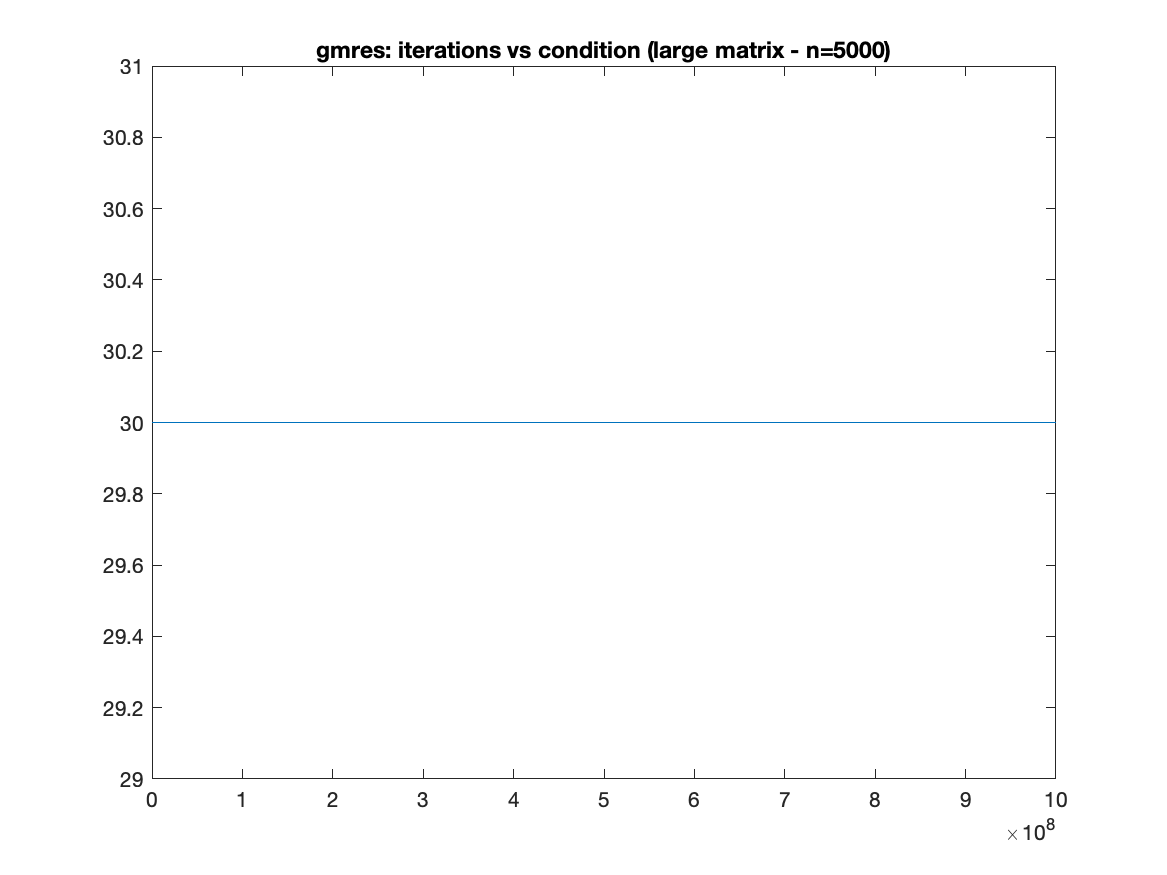
\includegraphics[width=\linewidth]{Plot/gmres_iter_lmat.png}
        \caption{Iterations with condition number with GMRES}
        \label{fig:image9}
    \end{minipage}
    \hspace{0.5cm} 
    \begin{minipage}[b]{0.5\linewidth}
        \centering
        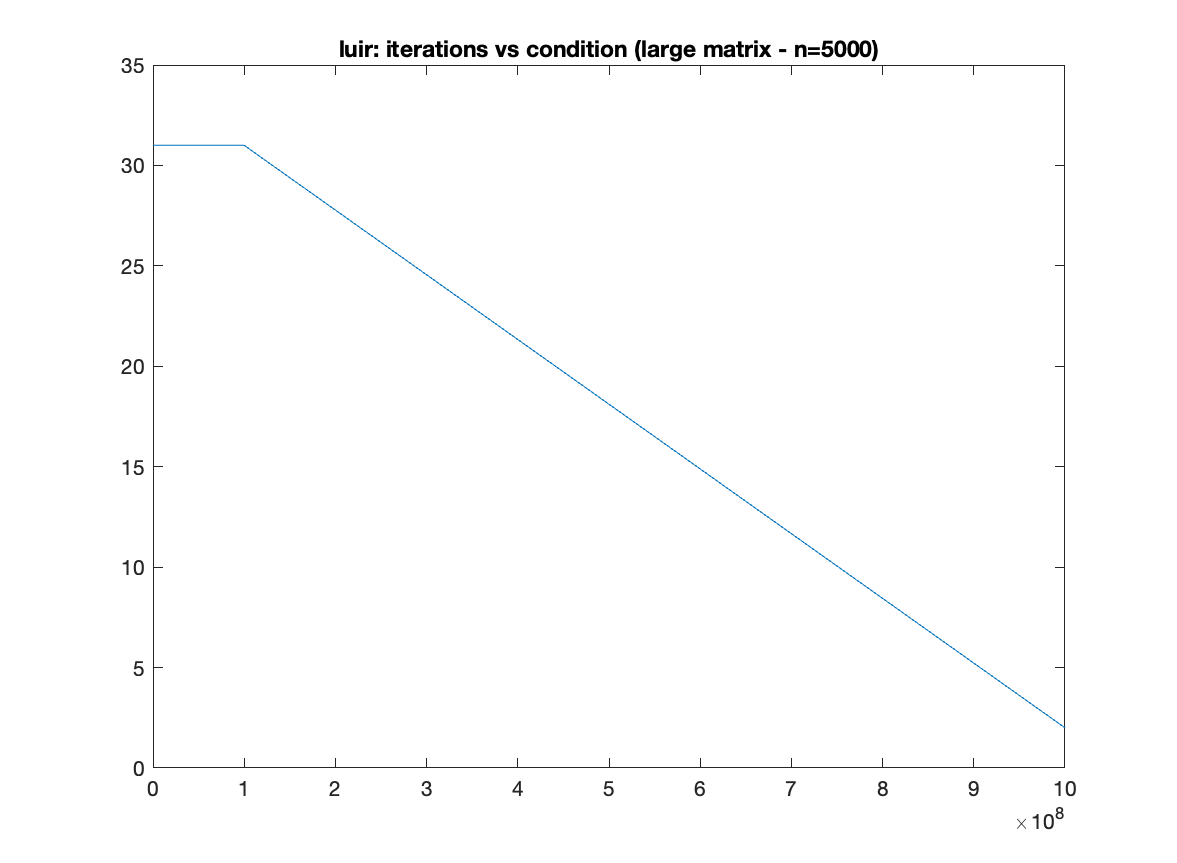
\includegraphics[width=\linewidth]{Plot/luir_iter_lmat.png}
        \caption{Iterations with condition number with LU-IR.}
        \label{fig:image10}
    \end{minipage}
\end{figure}
\newpage
\begin{figure}[ht]
     \begin{minipage}[b]{0.5\linewidth}
        \centering
   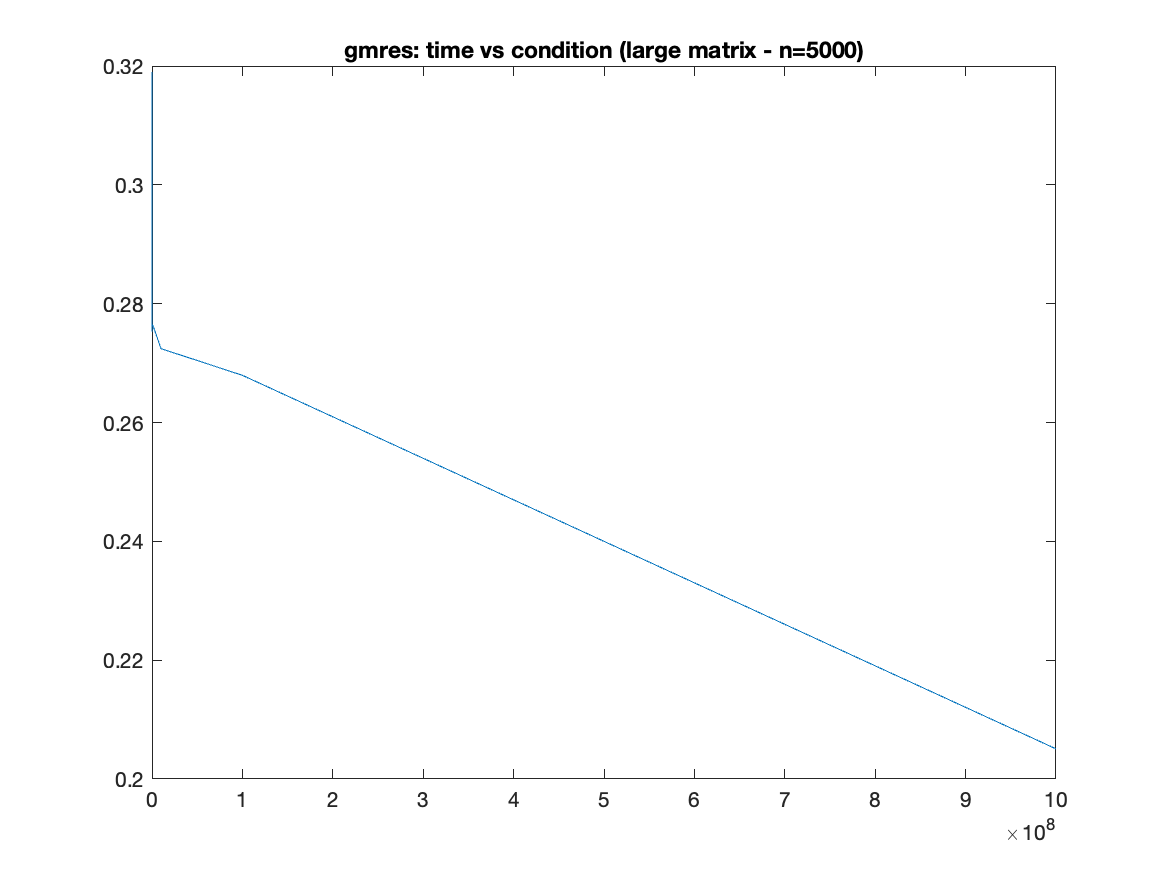
\includegraphics[width=\linewidth]{Plot/gmres_time_lmat.png}
        \caption{Time with condition number with GMRES}
        \label{fig:image11}
    \end{minipage}
    \hspace{0.5cm} 
    \begin{minipage}[b]{0.5\linewidth}
        \centering
        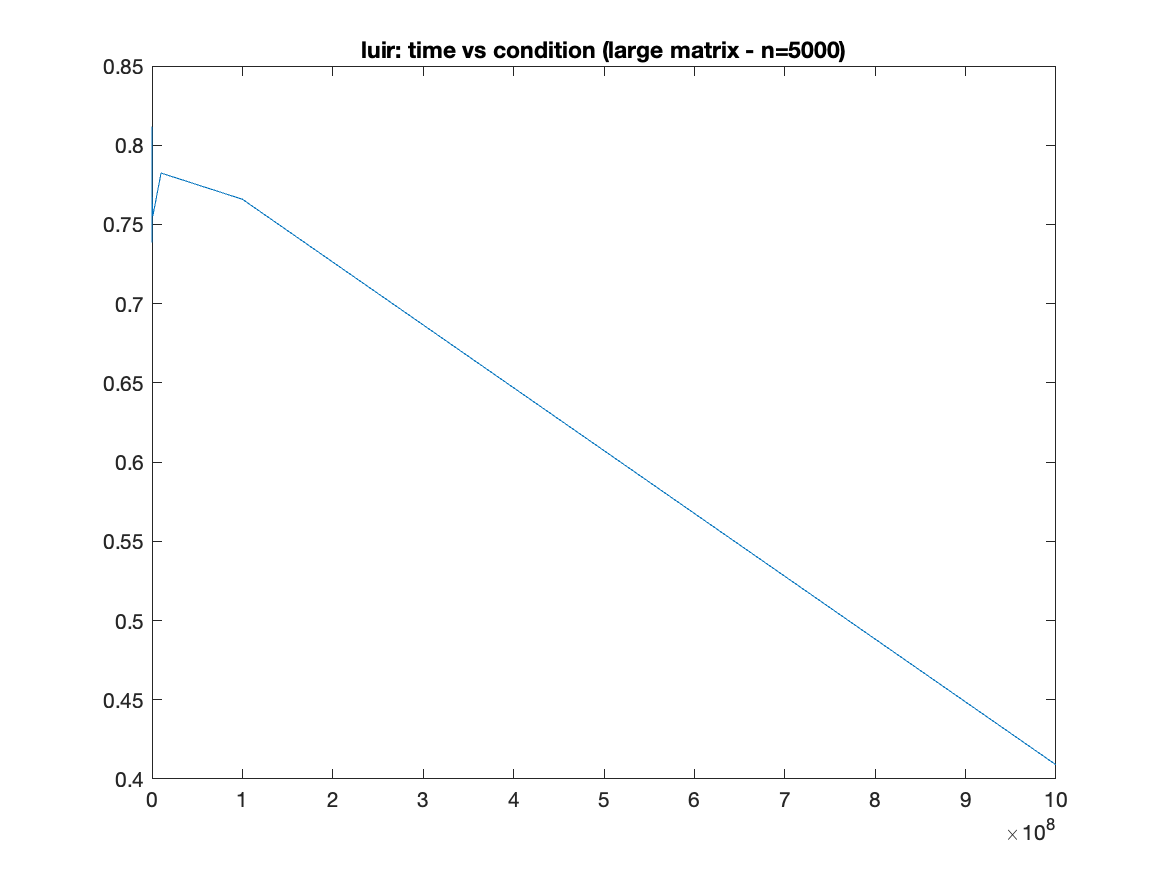
\includegraphics[width=\linewidth]{Plot/luir_time_lmat.png}
        \caption{Time with condition number with LU-IR.}
        \label{fig:image12}
    \end{minipage}
\end{figure}
\clearpage
\newpage
Matrices with high condition number:
\begin{lstlisting}[language=Matlab,caption=Matrix with high contional number]
sizes = [10,100,500,1000, 5000];
matrices = cell(size(sizes,2));
for i=1:size(sizes,2)
    matrices{i} = genMatrix(sizes(i), 1e9);
end

relresgm = zeros(size(matrices,2),1);
relreslu = zeros(size(matrices,2),1);
itergm = zeros(size(matrices,2),1);
iterlu = zeros(size(matrices,2),1);
timegm = zeros(size(matrices,2),1);
timelu = zeros(size(matrices,2),1);
flags = zeros(size(matrices,2),1);

for i = 1:size(matrices,2)
    b = rand(size(matrices{i},1),1);
    tic
    [x, flag, relres, iter] = gmres(matrices{i}, b, [], 1e-6, 30);
    timegm(i) = toc;
    relresgm(i) = relres;
    flags(i) = flag;
    itergm(i) = iter(2);

    tic
    [x, relres, iter] = iterref(matrices{i}, b);
    timelu(i) = toc;
    relreslu(i) = relres(size(relres,2));
    iterlu(i) = iter;
end

figure(1)
semilogy(sizes, relreslu);
title("luir: accuracy vs matrix size (high condition number)")
saveas(gcf,'luir_acc_hcond.png')
figure(2)
semilogy(sizes, relresgm);
title("gmres: accuracy vs matrix size (high condition number)")
saveas(gcf,'gmres_acc_hcond.png')

figure(3)
plot(sizes, iterlu);
title("luir: iterations vs matrix size (high condition number)")
saveas(gcf,'luir_iter_hcond.png')
figure(4)
plot(sizes, itergm);
title("gmres: iterations vs matrix size (high condition number)")
saveas(gcf,'luir_iter_hcond.png')

figure(5)
plot(sizes, timelu);
title("luir: time vs matrix size (low condition number)")
saveas(gcf,'luir_acc_lcond.png')
figure(6)
plot(sizes, timegm);
title("gmres: time vs matrix size (low condition number)")
saveas(gcf,'luir_acc_lcond.png')
   
\end{lstlisting}
With matrices with high condition number, we got results as below:
\begin{figure}[ht]
     \begin{minipage}[b]{0.5\linewidth}
        \centering
   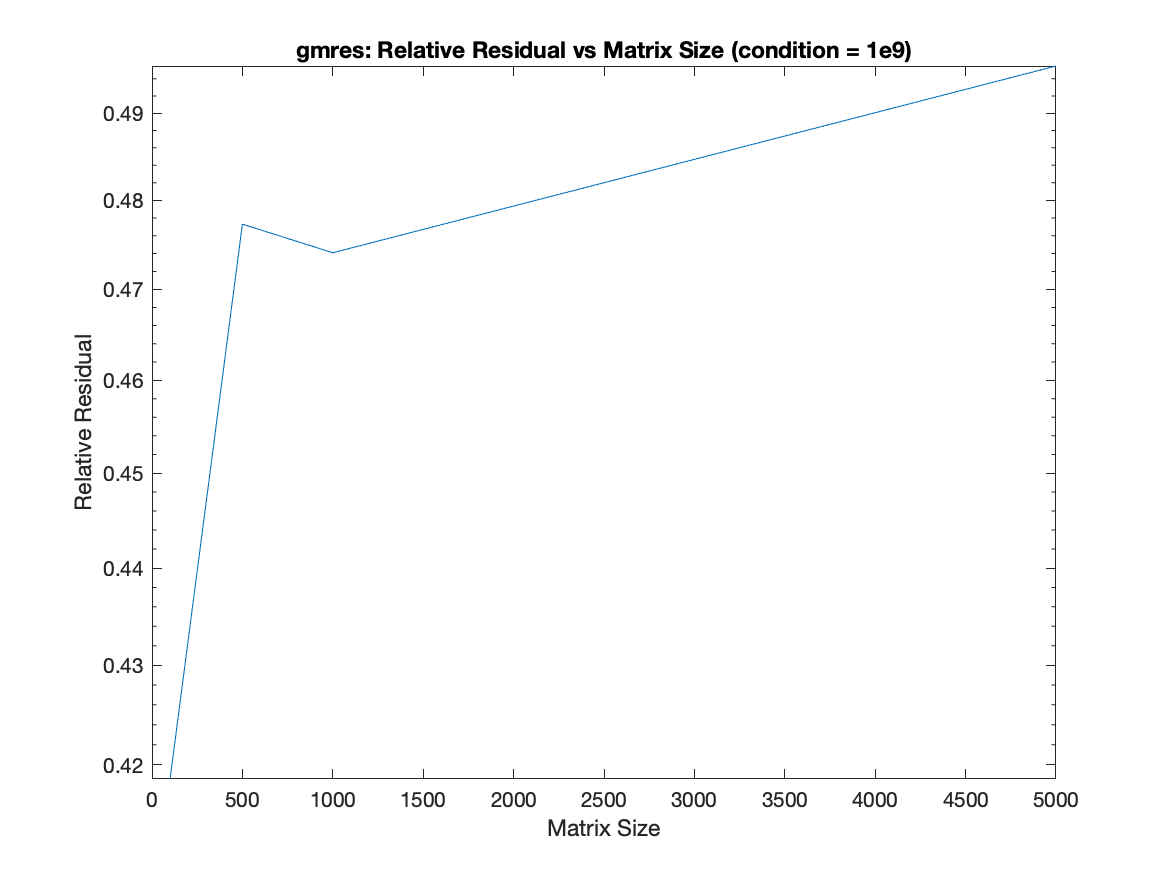
\includegraphics[width=\linewidth]{Plot/gmres_acc_hcond.png}
        \caption{Accuracy with size of matrix with GMRES}
        \label{fig:image13}
    \end{minipage}
    \hspace{0.5cm} 
    \begin{minipage}[b]{0.5\linewidth}
        \centering
        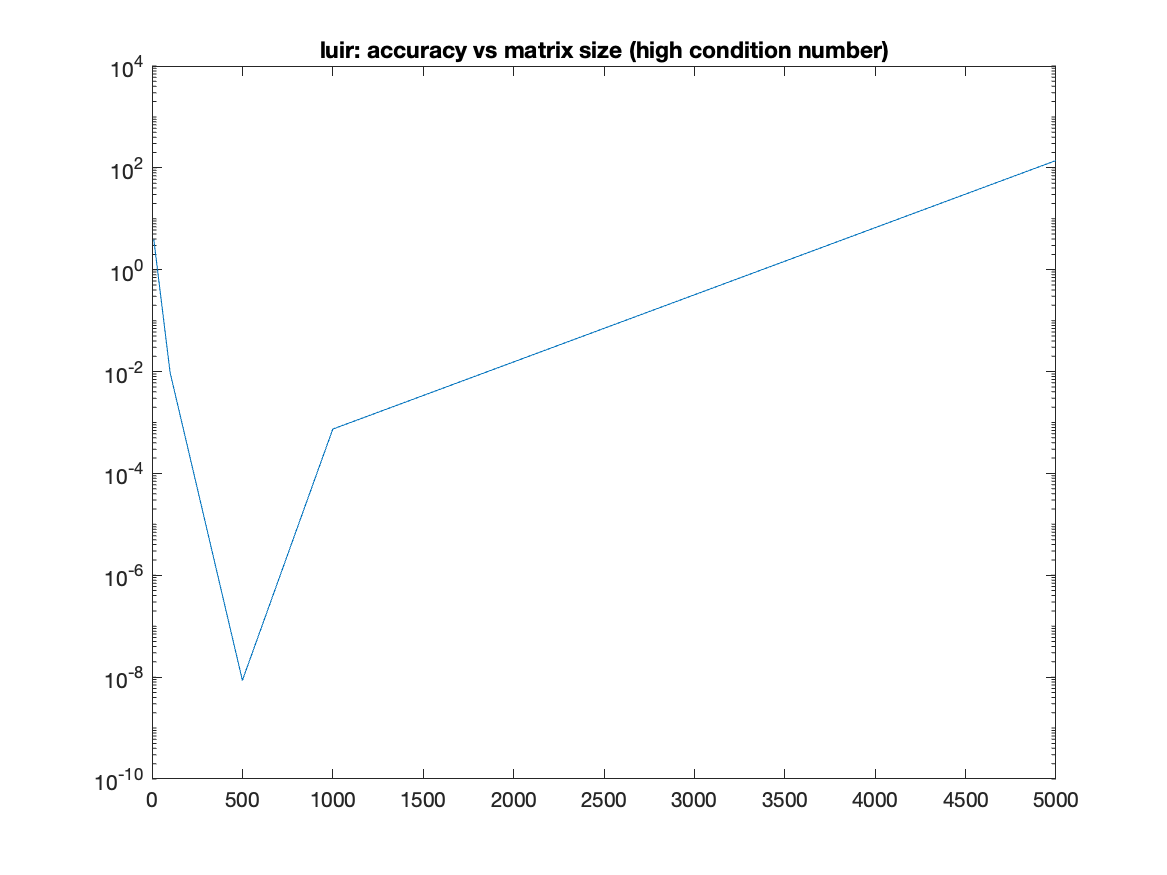
\includegraphics[width=\linewidth]{Plot/luir_acc_hcond.png}
        \caption{Accuracy with size of matrix with LU-IR.}
        \label{fig:image14}
    \end{minipage}
\end{figure}

\begin{figure}[ht]
     \begin{minipage}[b]{0.5\linewidth}
        \centering
   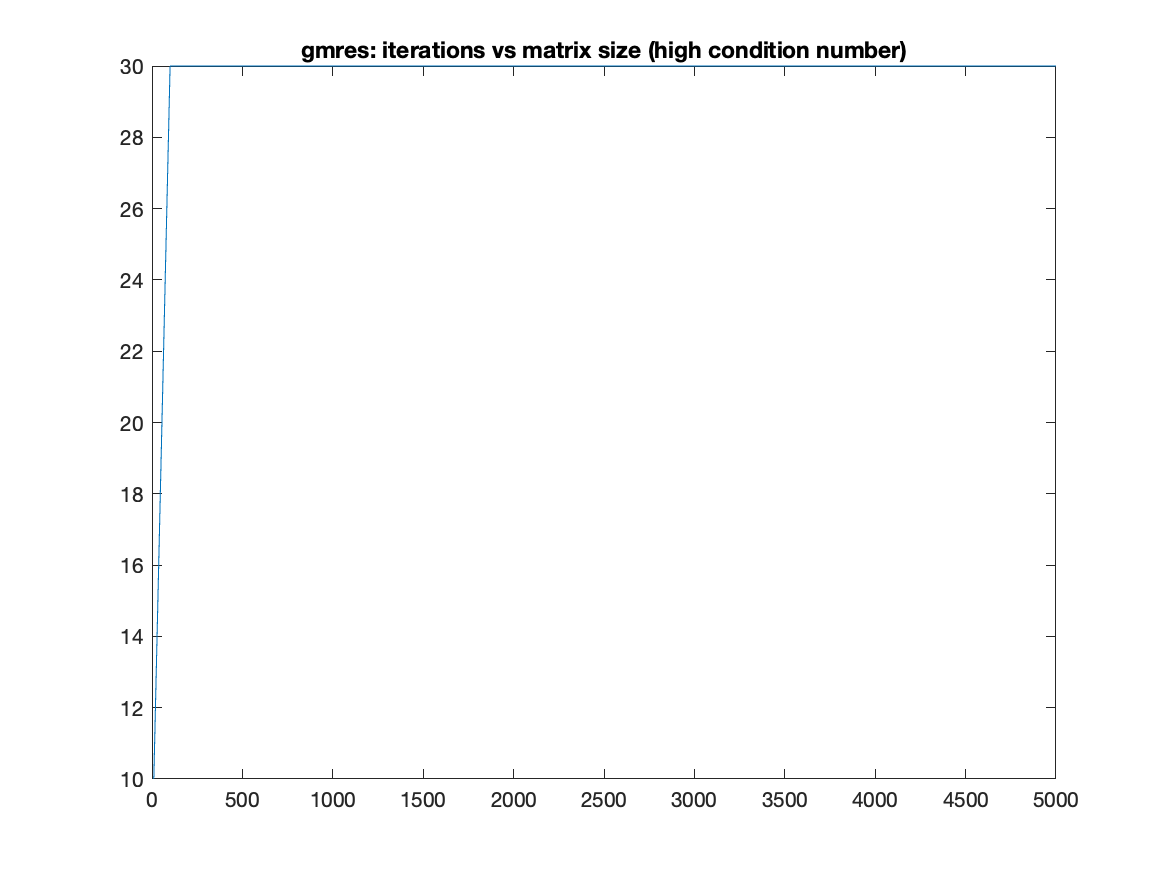
\includegraphics[width=\linewidth]{Plot/gmres_iter_hcond.png}
        \caption{Iterations with size of matrix with GMRES}
        \label{fig:image15}
    \end{minipage}
    \hspace{0.5cm} 
    \begin{minipage}[b]{0.5\linewidth}
        \centering
        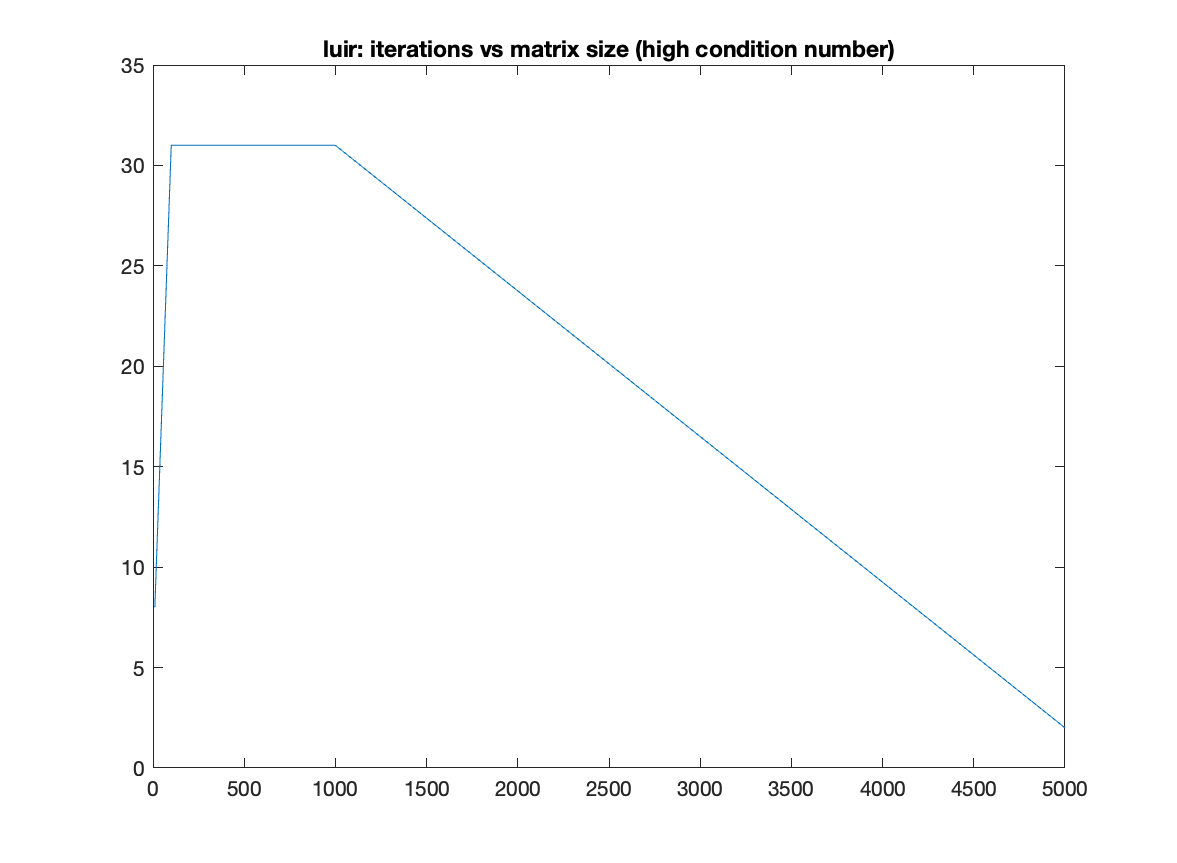
\includegraphics[width=\linewidth]{Plot/luir_iter_hcond.png}
        \caption{Iterations with size of matrix with LU-IR.}
        \label{fig:image16}
    \end{minipage}
\end{figure}
\newpage
\begin{figure}[ht]
     \begin{minipage}[b]{0.5\linewidth}
        \centering
   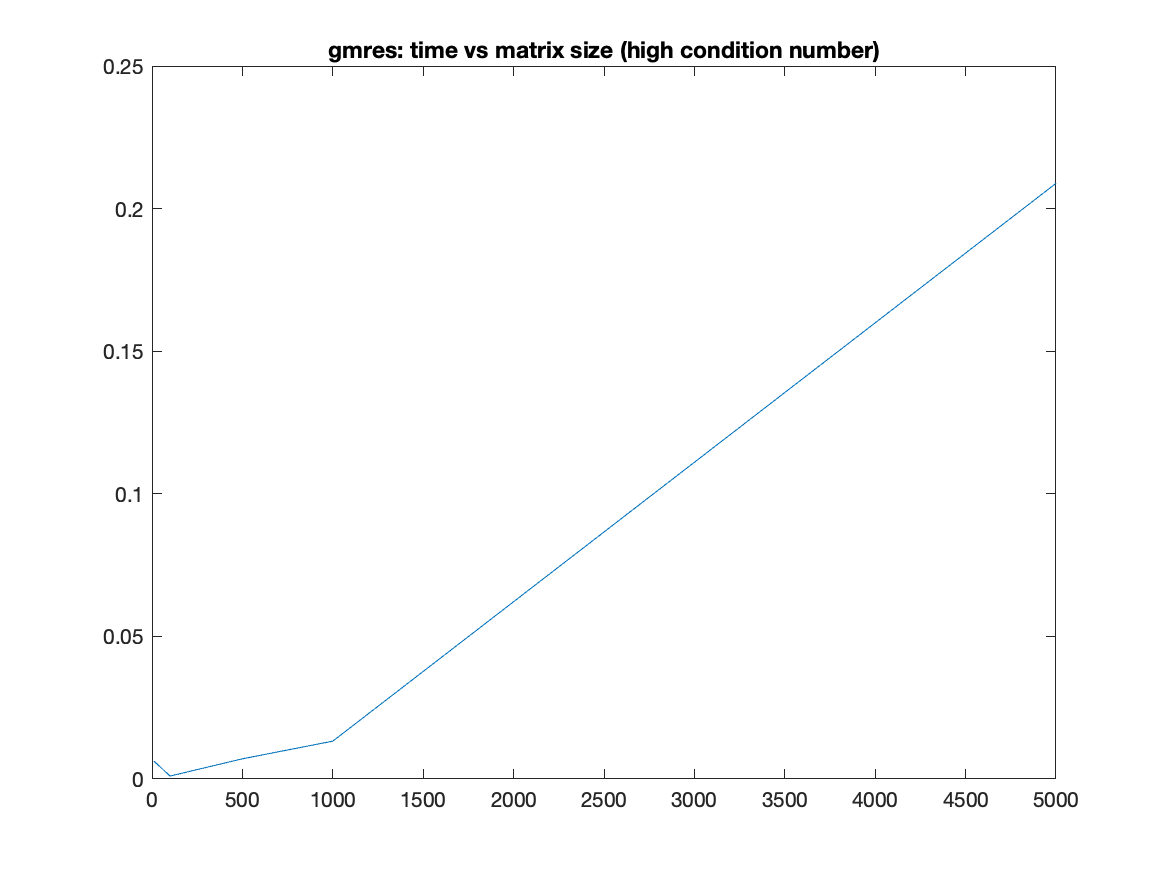
\includegraphics[width=\linewidth]{Plot/gmres_time_hcond.png}
        \caption{Time with size of matrix with GMRES}
        \label{fig:image17}
    \end{minipage}
    \hspace{0.5cm} 
    \begin{minipage}[b]{0.5\linewidth}
        \centering
        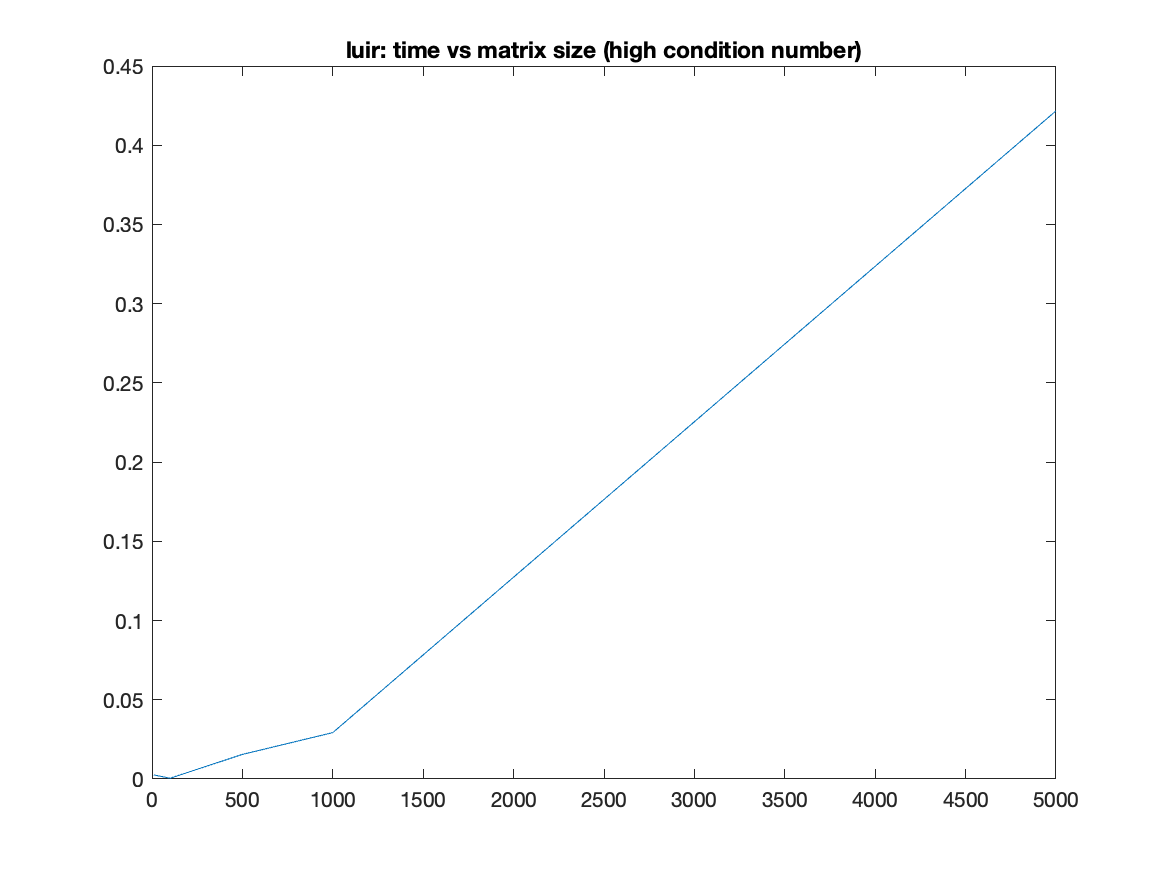
\includegraphics[width=\linewidth]{Plot/luir_time_hcond.png}
        \caption{Time with size of matrix with LU-IR.}
        \label{fig:image18}
    \end{minipage}
\end{figure}
\clearpage



Matrices with low condition number:
\begin{lstlisting}[language=matlab,caption=Matrix with low conditional number]
    sizes = [10,100,500,1000, 5000];
matrices = cell(size(sizes,2));
for i=1:size(sizes,2)
    matrices{i} = genMatrix(sizes(i), 1e2);
end

relresgm = zeros(size(matrices,2),1);
relreslu = zeros(size(matrices,2),1);
itergm = zeros(size(matrices,2),1);
iterlu = zeros(size(matrices,2),1);
timegm = zeros(size(matrices,2),1);
timelu = zeros(size(matrices,2),1);
flags = zeros(size(matrices,2),1);

for i = 1:size(matrices,2)
    b = rand(size(matrices{i},1),1);
    tic
    [x, flag, relres, iter] = gmres(matrices{i}, b, [], 1e-6, 30);
    timegm(i) = toc;
    relresgm(i) = relres;
    flags(i) = flag;
    itergm(i) = iter(2);

    tic
    [x, relres, iter] = iterref(matrices{i}, b);
    timelu(i) = toc;
    relreslu(i) = relres(size(relres,2));
    iterlu(i) = iter;
end

figure(1)
semilogy(sizes, relreslu);
title("luir: accuracy vs matrix size (low condition number)")
saveas(gcf,'luir_acc_lcond.png')
figure(2)
semilogy(sizes, relresgm);
title("gmres: accuracy vs matrix size (low condition number)")
saveas(gcf,'luir_acc_lcond.png')

figure(3)
plot(sizes, iterlu);
title("luir: iterations vs matrix size (low condition number)")
saveas(gcf,'luir_acc_lcond.png')
figure(4)
plot(sizes, itergm);
title("gmres: iterations vs matrix size (low condition number)")
saveas(gcf,'luir_acc_lcond.png')

figure(5)
plot(sizes, timelu);
title("luir: time vs matrix size (low condition number)")
saveas(gcf,'luir_acc_lcond.png')
figure(6)
plot(sizes, timegm);
title("gmres: time vs matrix size (low condition number)")
saveas(gcf,'luir_acc_lcond.png')

\end{lstlisting}
With matrices with low condition number as above, we got results as below:
\begin{figure}[ht]
     \begin{minipage}[b]{0.5\linewidth}
        \centering
   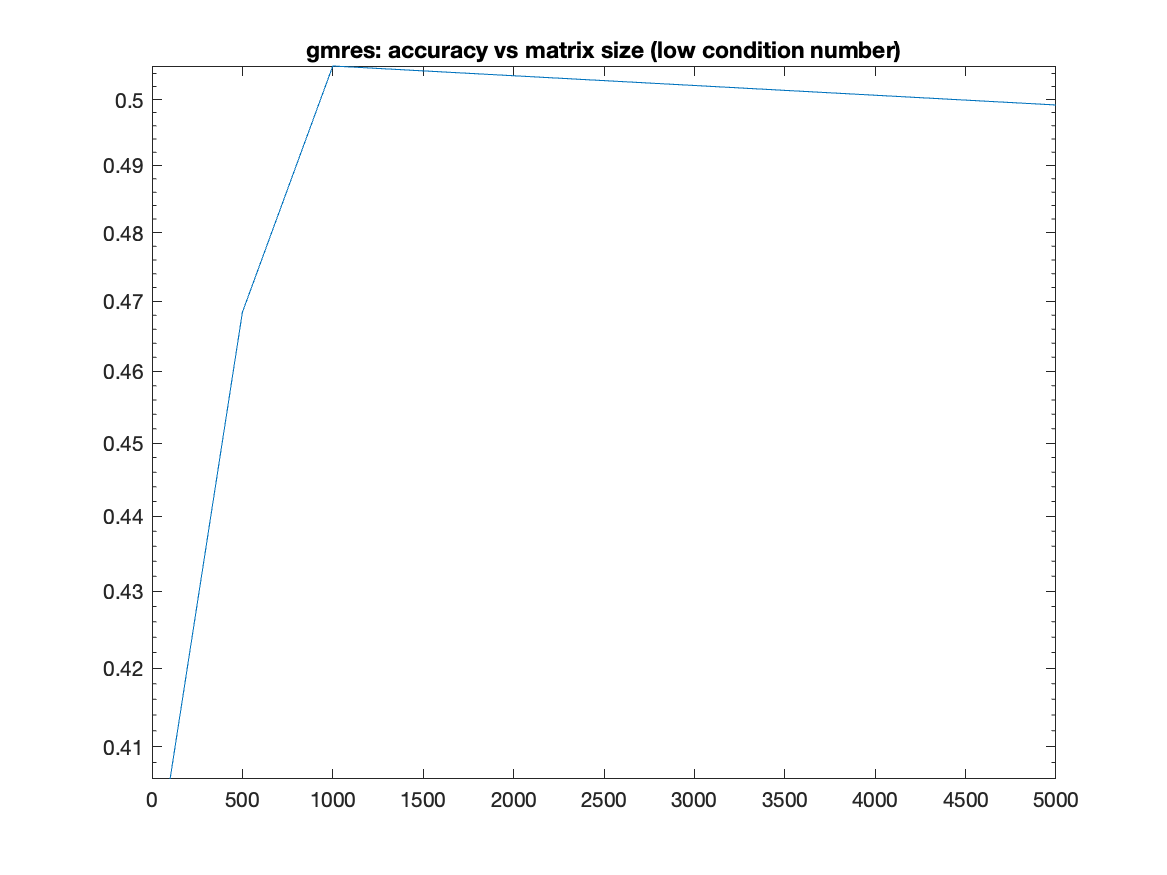
\includegraphics[width=\linewidth]{Plot/gmres_acc_lcond.png}
        \caption{Accuracy with size of matrix with GMRES}
        \label{fig:image19}
    \end{minipage}
    \hspace{0.5cm} 
    \begin{minipage}[b]{0.5\linewidth}
        \centering
        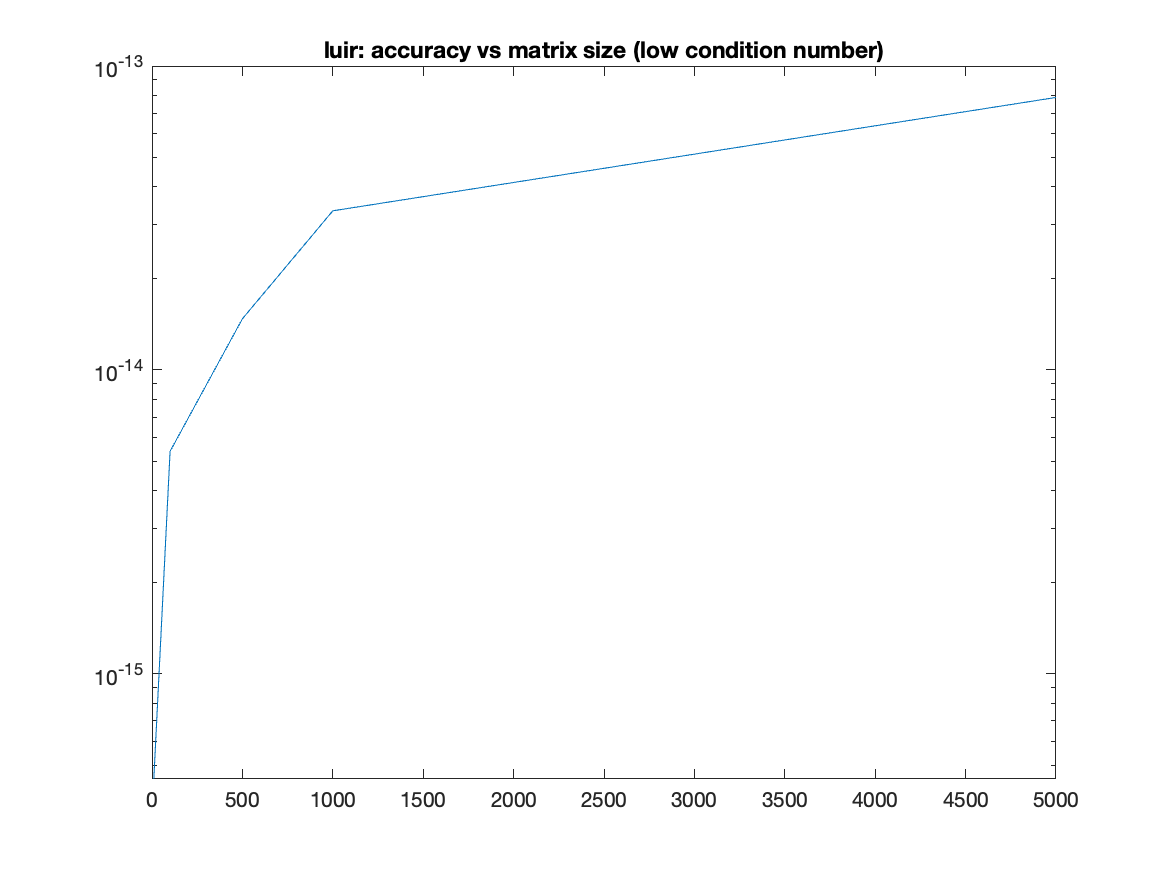
\includegraphics[width=\linewidth]{Plot/luir_acc_lcond.png}
        \caption{Accuracy with size of matrix with LU-IR.}
        \label{fig:image20}
    \end{minipage}
\end{figure}

\begin{figure}[ht]
     \begin{minipage}[b]{0.5\linewidth}
        \centering
   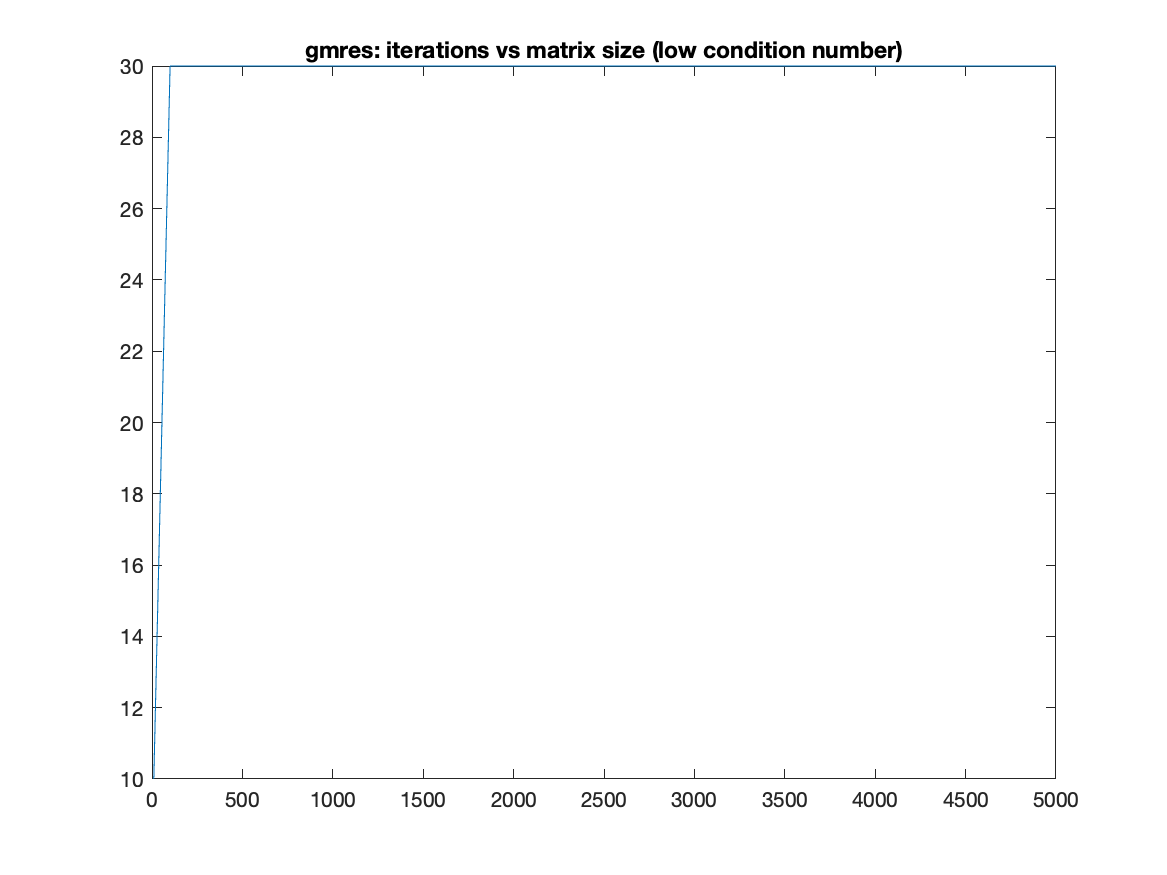
\includegraphics[width=\linewidth]{Plot/gmres_iter_lcond.png}
        \caption{Iterations with size of matrix with GMRES}
        \label{fig:image21}
    \end{minipage}
    \hspace{0.5cm} 
    \begin{minipage}[b]{0.5\linewidth}
        \centering
        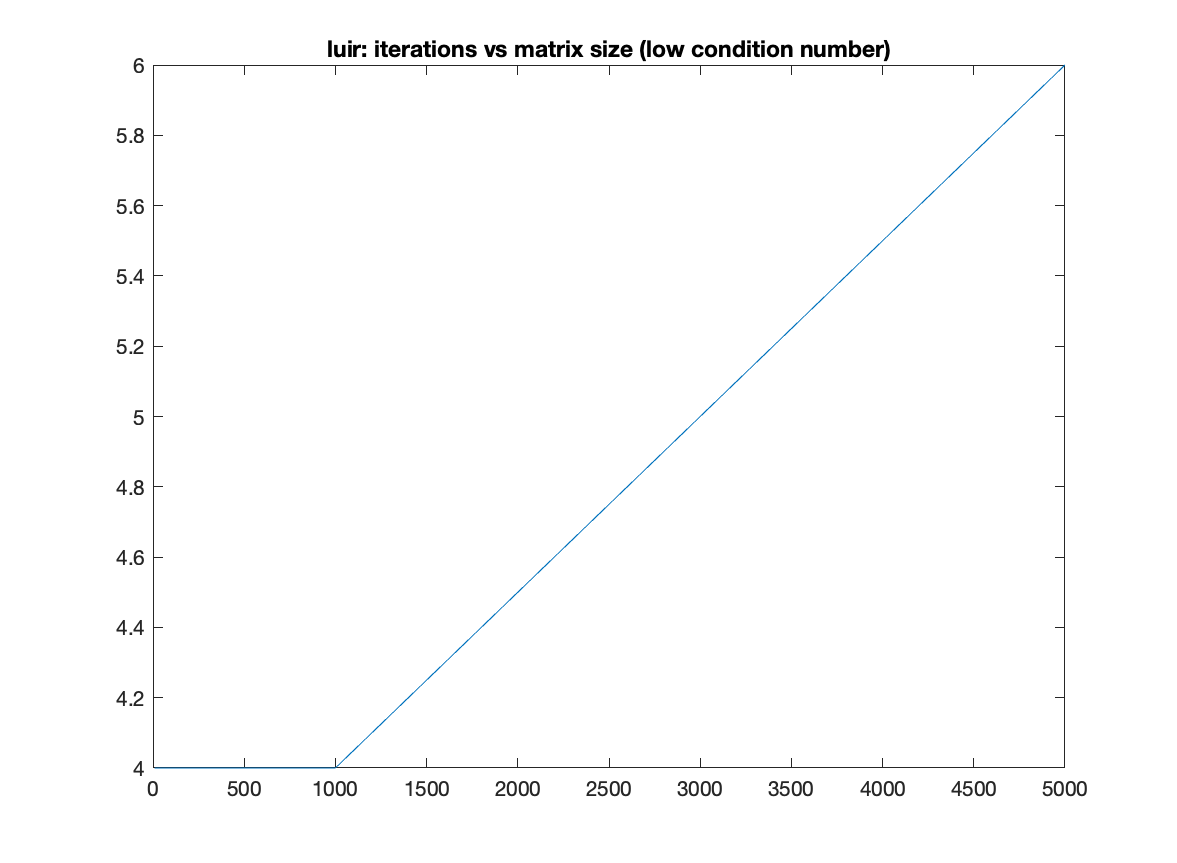
\includegraphics[width=\linewidth]{Plot/luir_iter_lcond.png}
        \caption{Iterations with size of matrix with LU-IR.}
        \label{fig:image22}
    \end{minipage}
\end{figure}
\newpage
\begin{figure}[ht]
     \begin{minipage}[b]{0.5\linewidth}
        \centering
   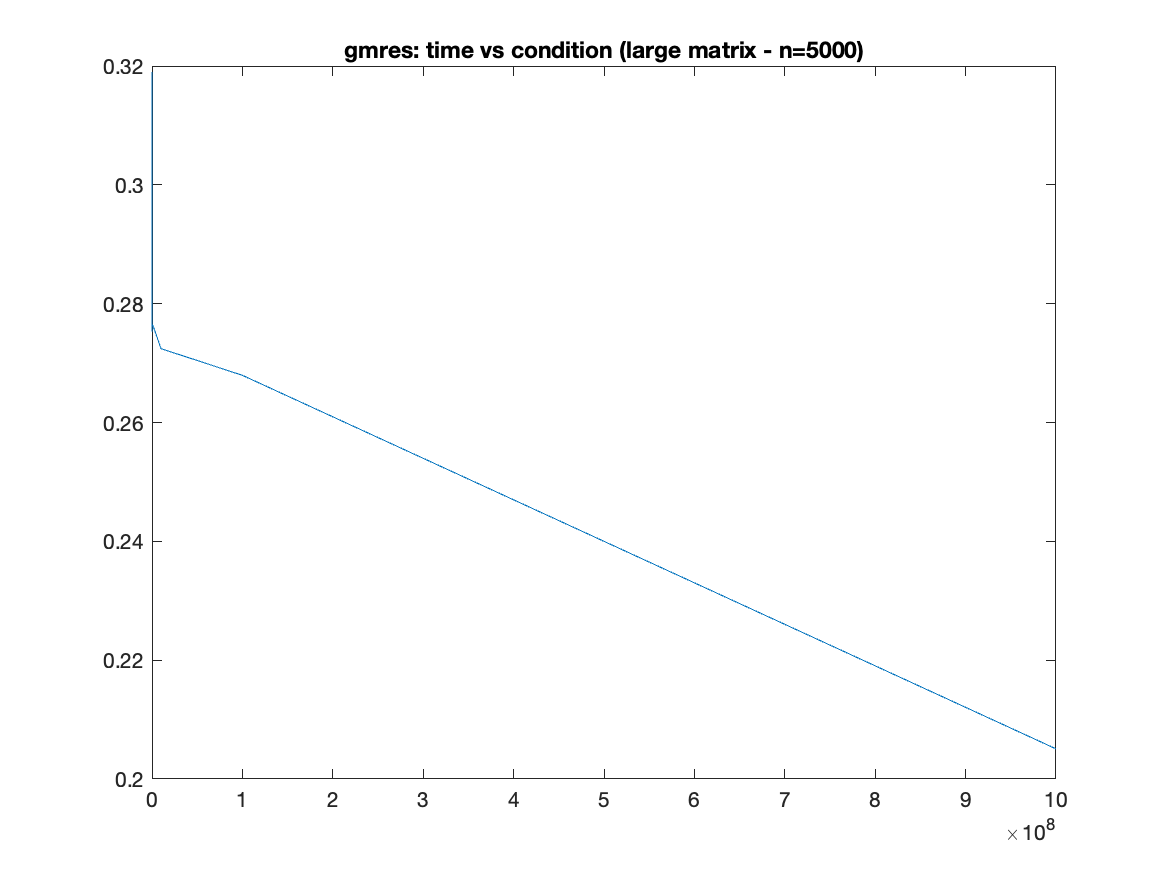
\includegraphics[width=\linewidth]{Plot/gmres_time_lmat.png}
        \caption{Time with size of matrix with GMRES}
        \label{fig:image23}
    \end{minipage}
    \hspace{0.5cm} 
    \begin{minipage}[b]{0.5\linewidth}
        \centering
        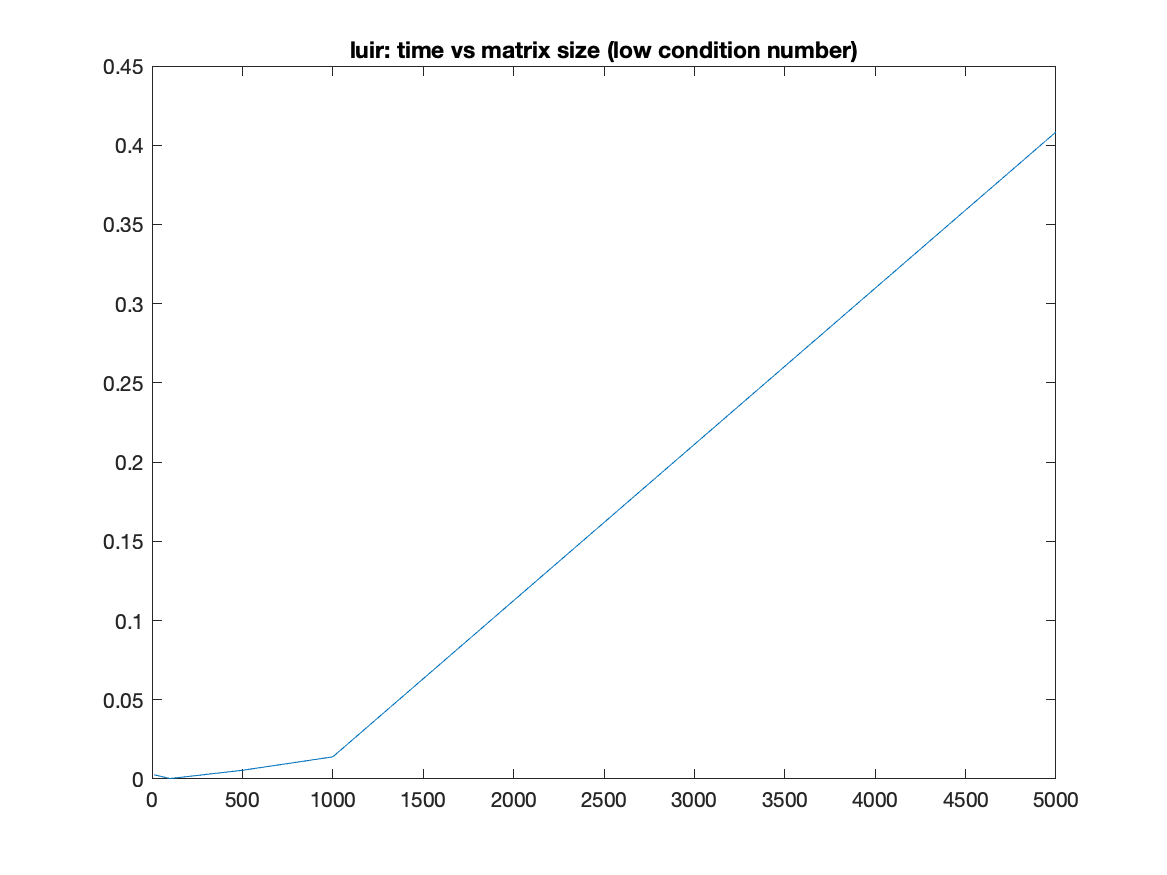
\includegraphics[width=\linewidth]{Plot/luir_time_lcond.png}
        \caption{Time with size of matrix with LU-IR.}
        \label{fig:image24}
    \end{minipage}
\end{figure}
\clearpage